\section{Erstiwochenende -- Was dann geschah ist unglaublich}
\textbf{Ihr könnt euch vielleicht noch nicht sehr viel unter dem "Erstiwochenende" vorstellen.
	Ist das ein Wochenende, an dem wir noch mehr lernen dürfen, als ohnehin schon?
	Oder schießen wir uns zwei Tage aus dem Leben?
	Hier ein kleiner Erfahrungsbericht.}

	% XXX Jedes Jahr Ersti-WE-Termin aktualisieren!
\textbf{\emph{Hinweis:}
% Das Erstiwochenende findet dieses Semester vom 13.11. bis zum 15.11.\ statt. (Verbindliche) Anmeldung in der Fachschaft. Tickets gibt es auch in den Spielen der O-Woche zu gewinnen; wir freuen uns auf euch!
Das Erstiwochenende findet voraussichtlich im nächsten Semester statt. Weitere Infos folgen; wir freuen uns auf euch!
}
\begin{multicols*}{2}
\subsection{Freitag, 15:00 Uhr}
Eine zunächst unscheinbare Gruppe Physiker steht am Hauptbahnhof.
Kaum ein Passant nahm Notiz von den Karohemden und Filzpullovern, die etwa eine Dreiviertelstunde zu früh am Hauptbahnhof standen.

What?
Eine Dreiviertelstunde?
Wie kann das sein?

Entgegen seiner Natur hat sich der Autor dieses Textes (also „Ich“) für einen Termin entschieden, der dafür sorgen sollte, dass alle dreißig Erstis pünktlich zum Bus erscheinen, der sie in ein unbekanntes Land vor gar nicht allzu langer Zeit führen sollte.

Der letzte Student kam um kurz nach halb vier.
Der Organisator (Ich) hatte also Recht behalten, würdigte der Tatsache aber keine Erwähnung, wohl wissend, dass die anderen ihn um seine organisatorischen Fähigkeiten beneideten.

Er selbst war natürlich auch nicht rechtzeitig da.

\subsection{Freitag, später}
Nach der Ankunft in einer ortsnahen, 500~Einwohner starken Metropole stand zunächst ein kurzes Einfinden im neu besetzten Gebiet auf dem Plan.
Die Zimmer wurden wild gemischt (Stand jetzt, 9~Monate später: Es hat auf der letzten Fahrt dadurch keiner das Recht auf Kindergeld erworben) bezogen.

Danach wurde die äußere Umgebung der bezogenen Residenz erkundet (Näheres dazu müsst ihr allerdings selbst auf der Fahrt in Erfahrung bringen).
Essen gab es auch noch und abends wurde dann eventuell auch noch ein klitzekleines bisschen getrunken.
An Genaueres kann ich mich aber nicht mehr erinnern.

\begin{center}
	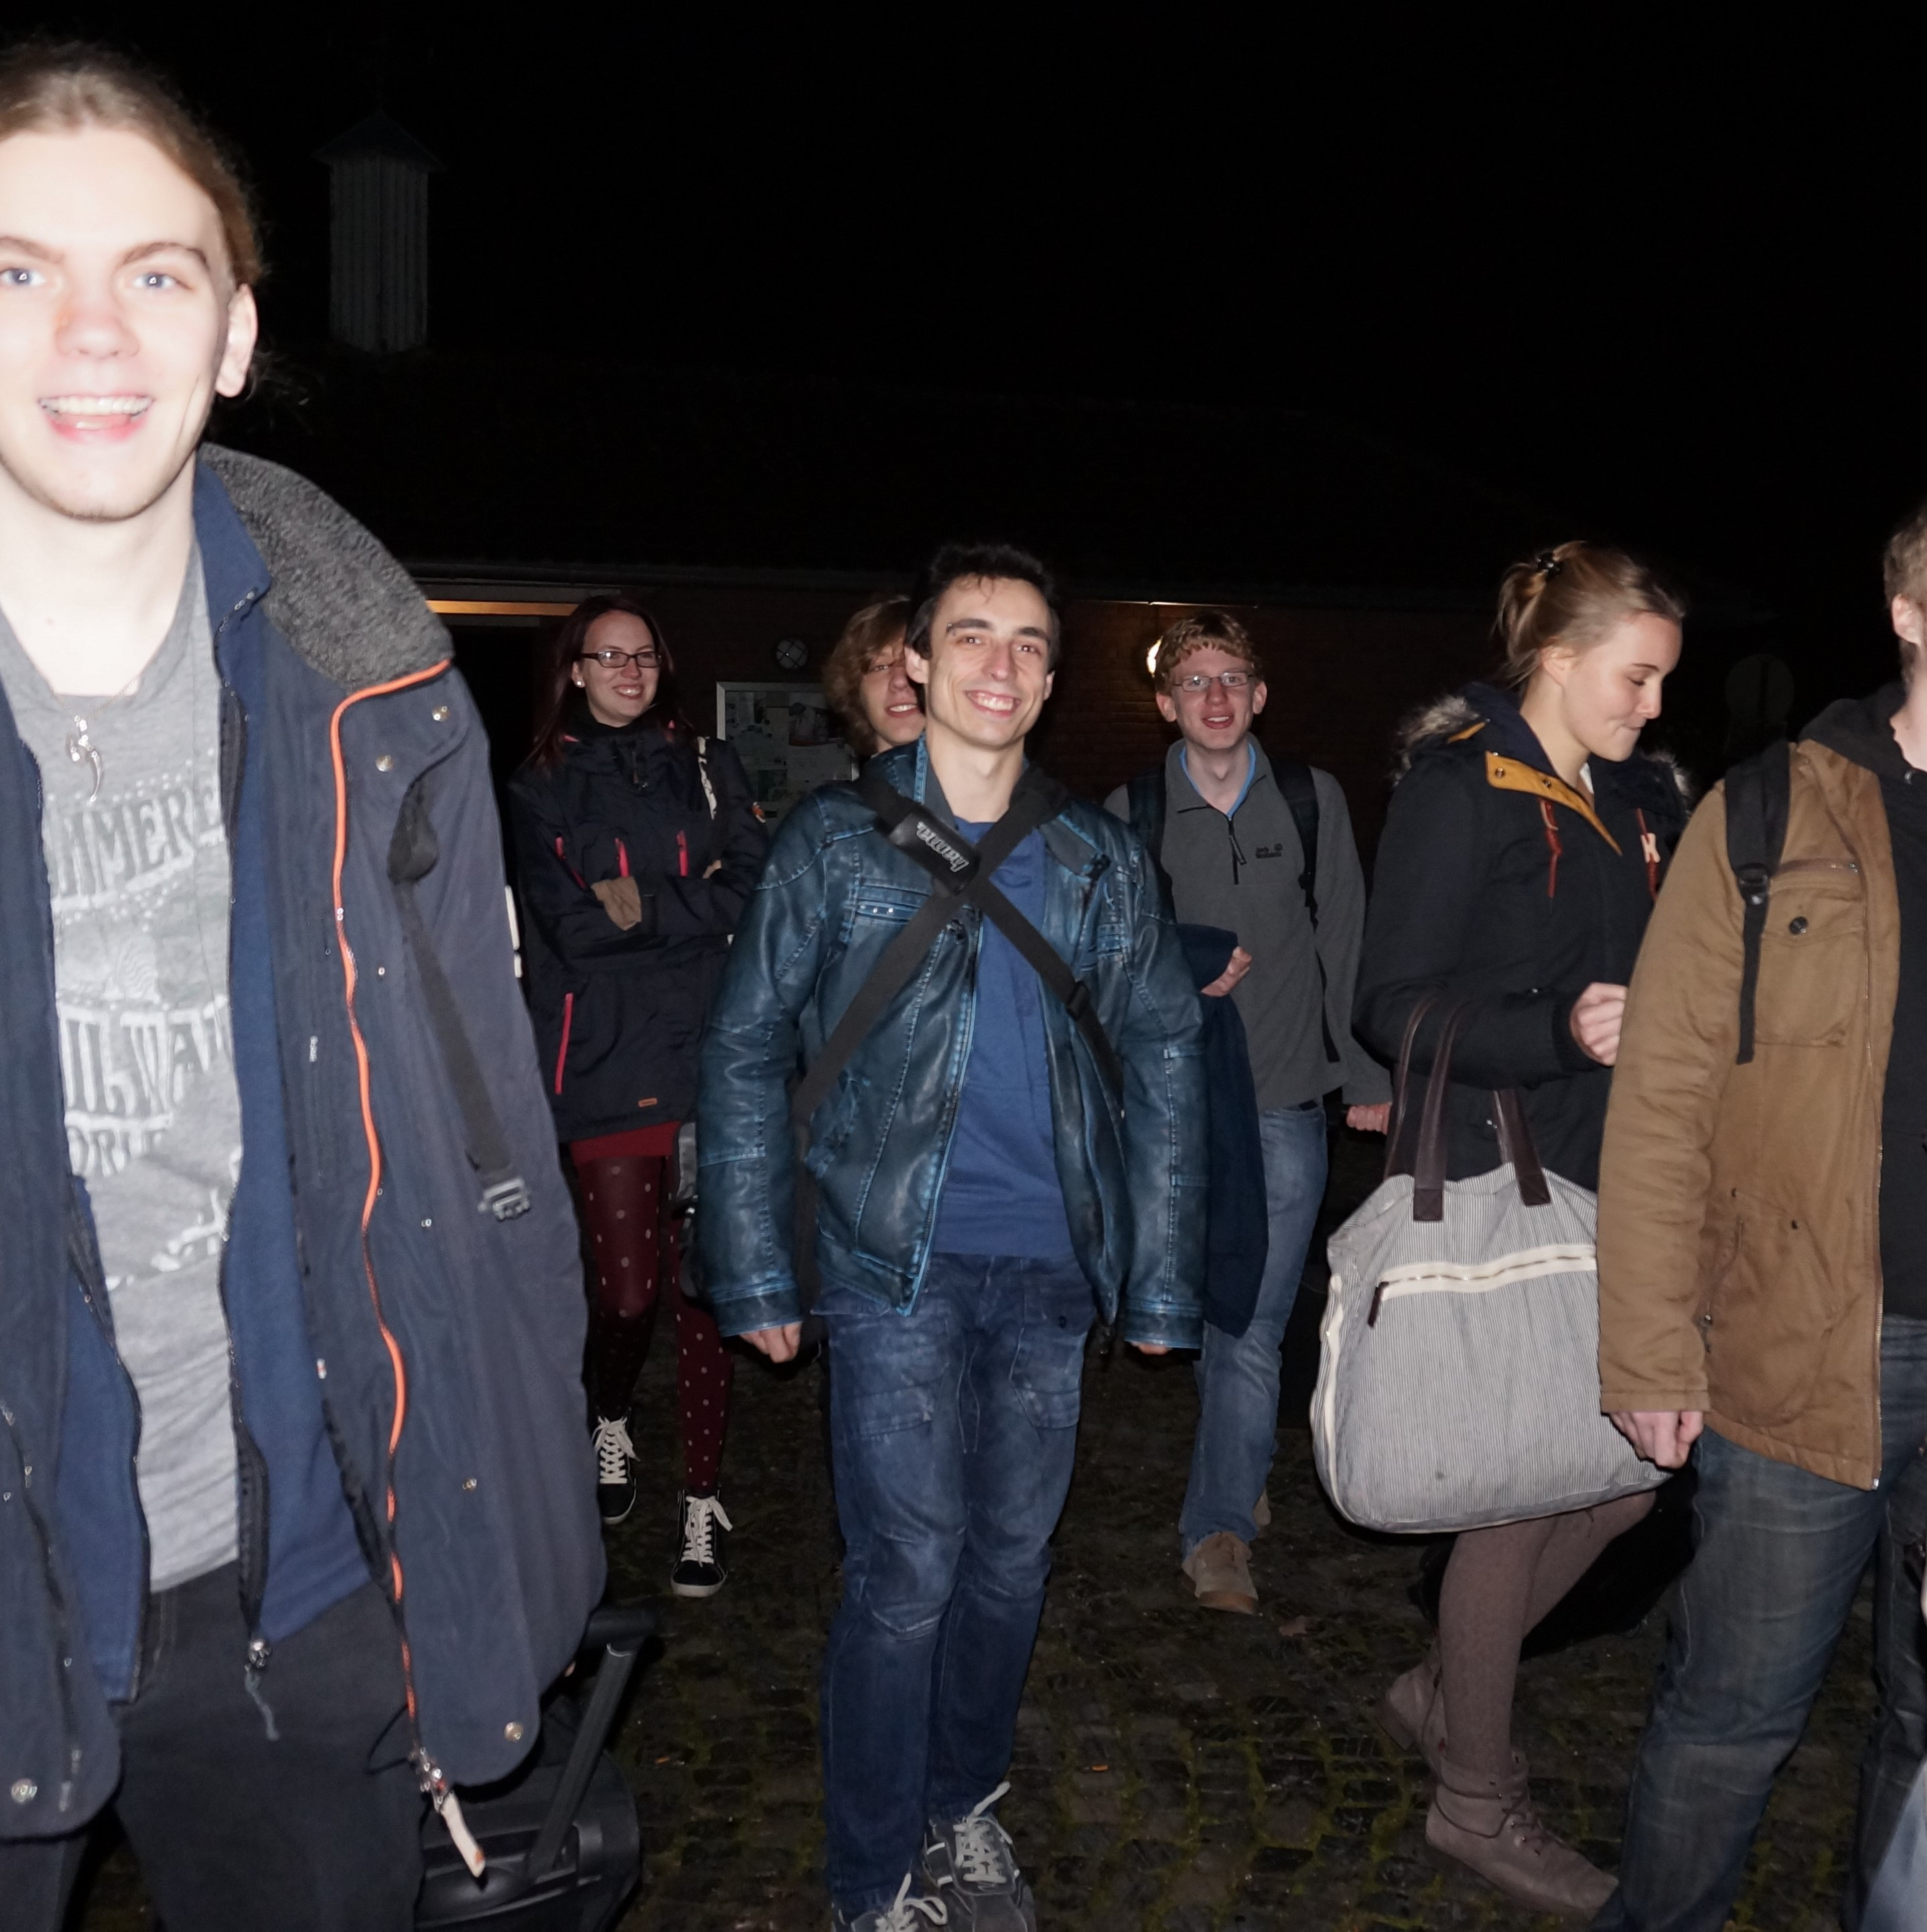
\includegraphics[width=\columnwidth]{res/erstiwe/ankunft_cropped.jpg}
\end{center}

\subsection{Samstag, etwas zu früh}
Leider musste die Fachschaft die eine oder andere Schlafgewohnheit am Wochenende durchbrechen, schließlich ist das Frühstück in einer Herberge noch nie langschläferfreundlich serviert worden.
So saßen am Morgen ein paar verschlafene Köpfe, aber auch ein paar Frühaufsteher, die sich schon angeregt unterhielten, zusammen am Frühstückstisch.

Da nach dem Frühstück ein wenig Freizeit wartete, haben sich ein paar Vollblutstudenten noch einmal hingelegt.
Ansonsten bestand auch die Möglichkeit, die Ortschaft zu besichtigen.
Die wohl interessanteste Sehenswürdigkeit dürfte dabei das Fuselregal im Supermarkt gewesen sein.

Da im Laufe der Zeit der Wissensdurst der Erstis gestiegen ist (schon \SI{24}{\hour} ohne Zettelrechnen!) hat ein Fachschaftler einen superschönen Vortrag zum Thema Hochschulpolitik vorbereitet.
Wer diesen unbedingt wieder vergessen wollte, war mit einem vorigen Ortsbesuch inklusive Supermarkt also gut beraten.

Wer konnte, durfte am Klavier auch einen zum Besten geben.
Wer es nicht konnte, durfte es auch -- wir sind der Meinung, dass jeder die Freiheit dazu haben sollte, sich bei Kommilitonen unbeliebt zu machen.

\begin{center}
	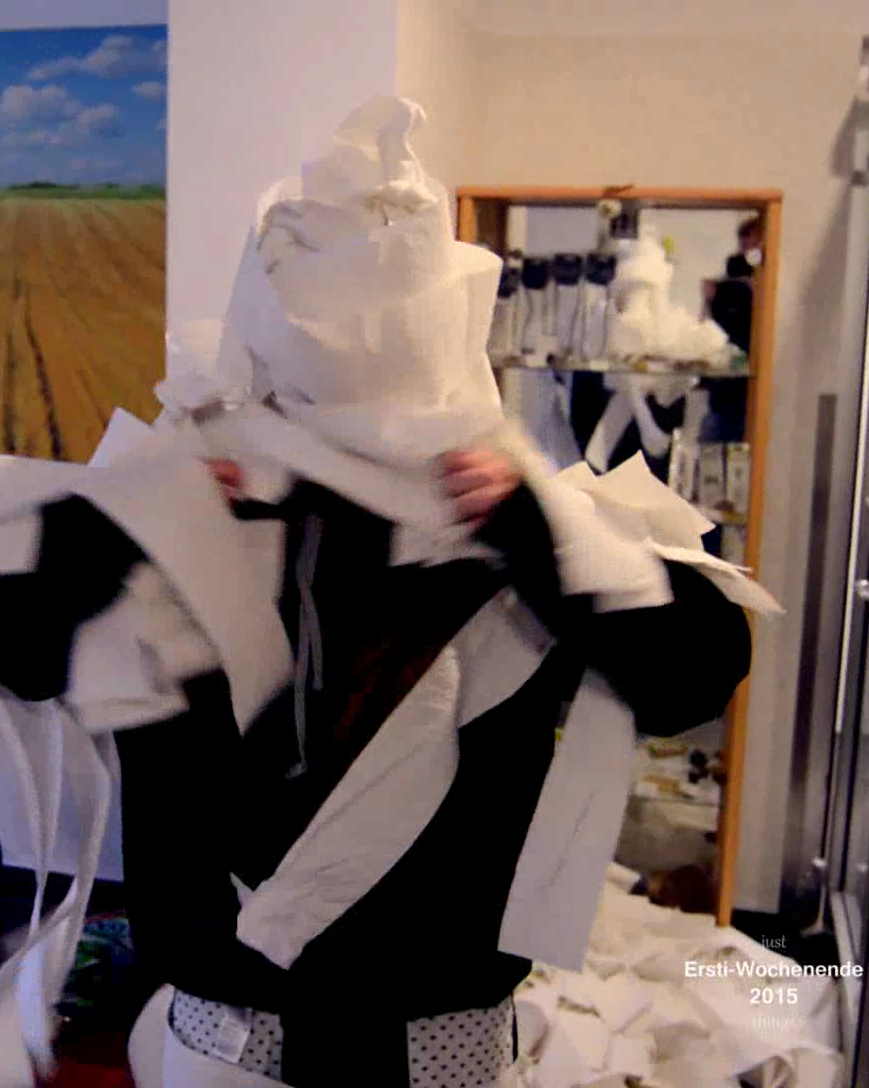
\includegraphics[width=\columnwidth]{res/erstiwe/klopapier-mumie.png}
\end{center}

\subsection{Samstag, etwas zu spät}
Mit kleiner Verzögerung stand das nächste Highlight auf der Tagesordnung:
Das Chaosspiel.
Der Name sagt euch in etwa so viel, wie wir euch vorher wissen lassen wollen, nämlich ungefähr nichts.
Viel Gewusel, aber ein großer Spaß (auch für die Fachschaftler).
Da das Spiel ein wenig Zeit in Anspruch nimmt, wird auch hier das Bier nicht unter Verschluss gehalten.

Nebst weiterer Programmpunkte begann zum späteren Abend hin ein völlig ungeplantes eventuelles klitzekleines Besäufnis.
Es wurde getanzt und gefeiert, die Unterkunft wurde auseinandergenommen (aber stehengelassen).
Zu später Stunde kommen Überlegungen auf, dass es womöglich angenehmer sein könnte, gar nicht zu schlafen, anstatt 

\subsection{Sonntag, unchristlich früh}
aufzustehen.
Extra für diesen Sonntag muss eine neue Uhrzeit erfunden worden sein.
Ein harmonisches Orchester aus Kochtöpfen und Handyweckern holte die Studenten wunderbar sanft aus einem friedlichen Schlummer.
Nichts anderes als eine Gruppe fröhlich strahlender Studenten konnte man im Frühstückssaal erwarten.

Nach der Erkenntnis, dass das Wochenende sich dem Ende neigte, wich das Lächeln jedoch einer wehmütigen Träne.
Würden sie jemals wieder solch eine Freude verspüren können?
Oder überhaupt Freude?
Zwar sprach es keiner an, doch war dem Organisator (Mir) klar, dass es genau das sein musste, was jedem Einzelnen durch den Kopf ging.
Am frühen Nachmittag erreichten wir schließlich wieder unseren Ausgangspunkt, ironischerweise eine Dreiviertelstunde zu spät. 

% XXX Jedes Jahr Ersti-WE-Termin aktualisieren!
Das Erstiwochenende ist ein wirklich schönes Erlebnis und lässt euch (wie auch in der O-Woche) schnell neue Kontakte knüpfen und Freundschaften aufbauen.
% Euer Erstiwochenende findet am \textbf{13.--15.~November} statt; Dieses Jahr \textbf{reisen wir an die Weser}, packt also eure Badesachen ein und meldet euch bei der Fachschaft an, solange noch Plätze verfügbar sind :)

\fibelsig{Fernando}
\vspace{3ex}
\begin{center}
	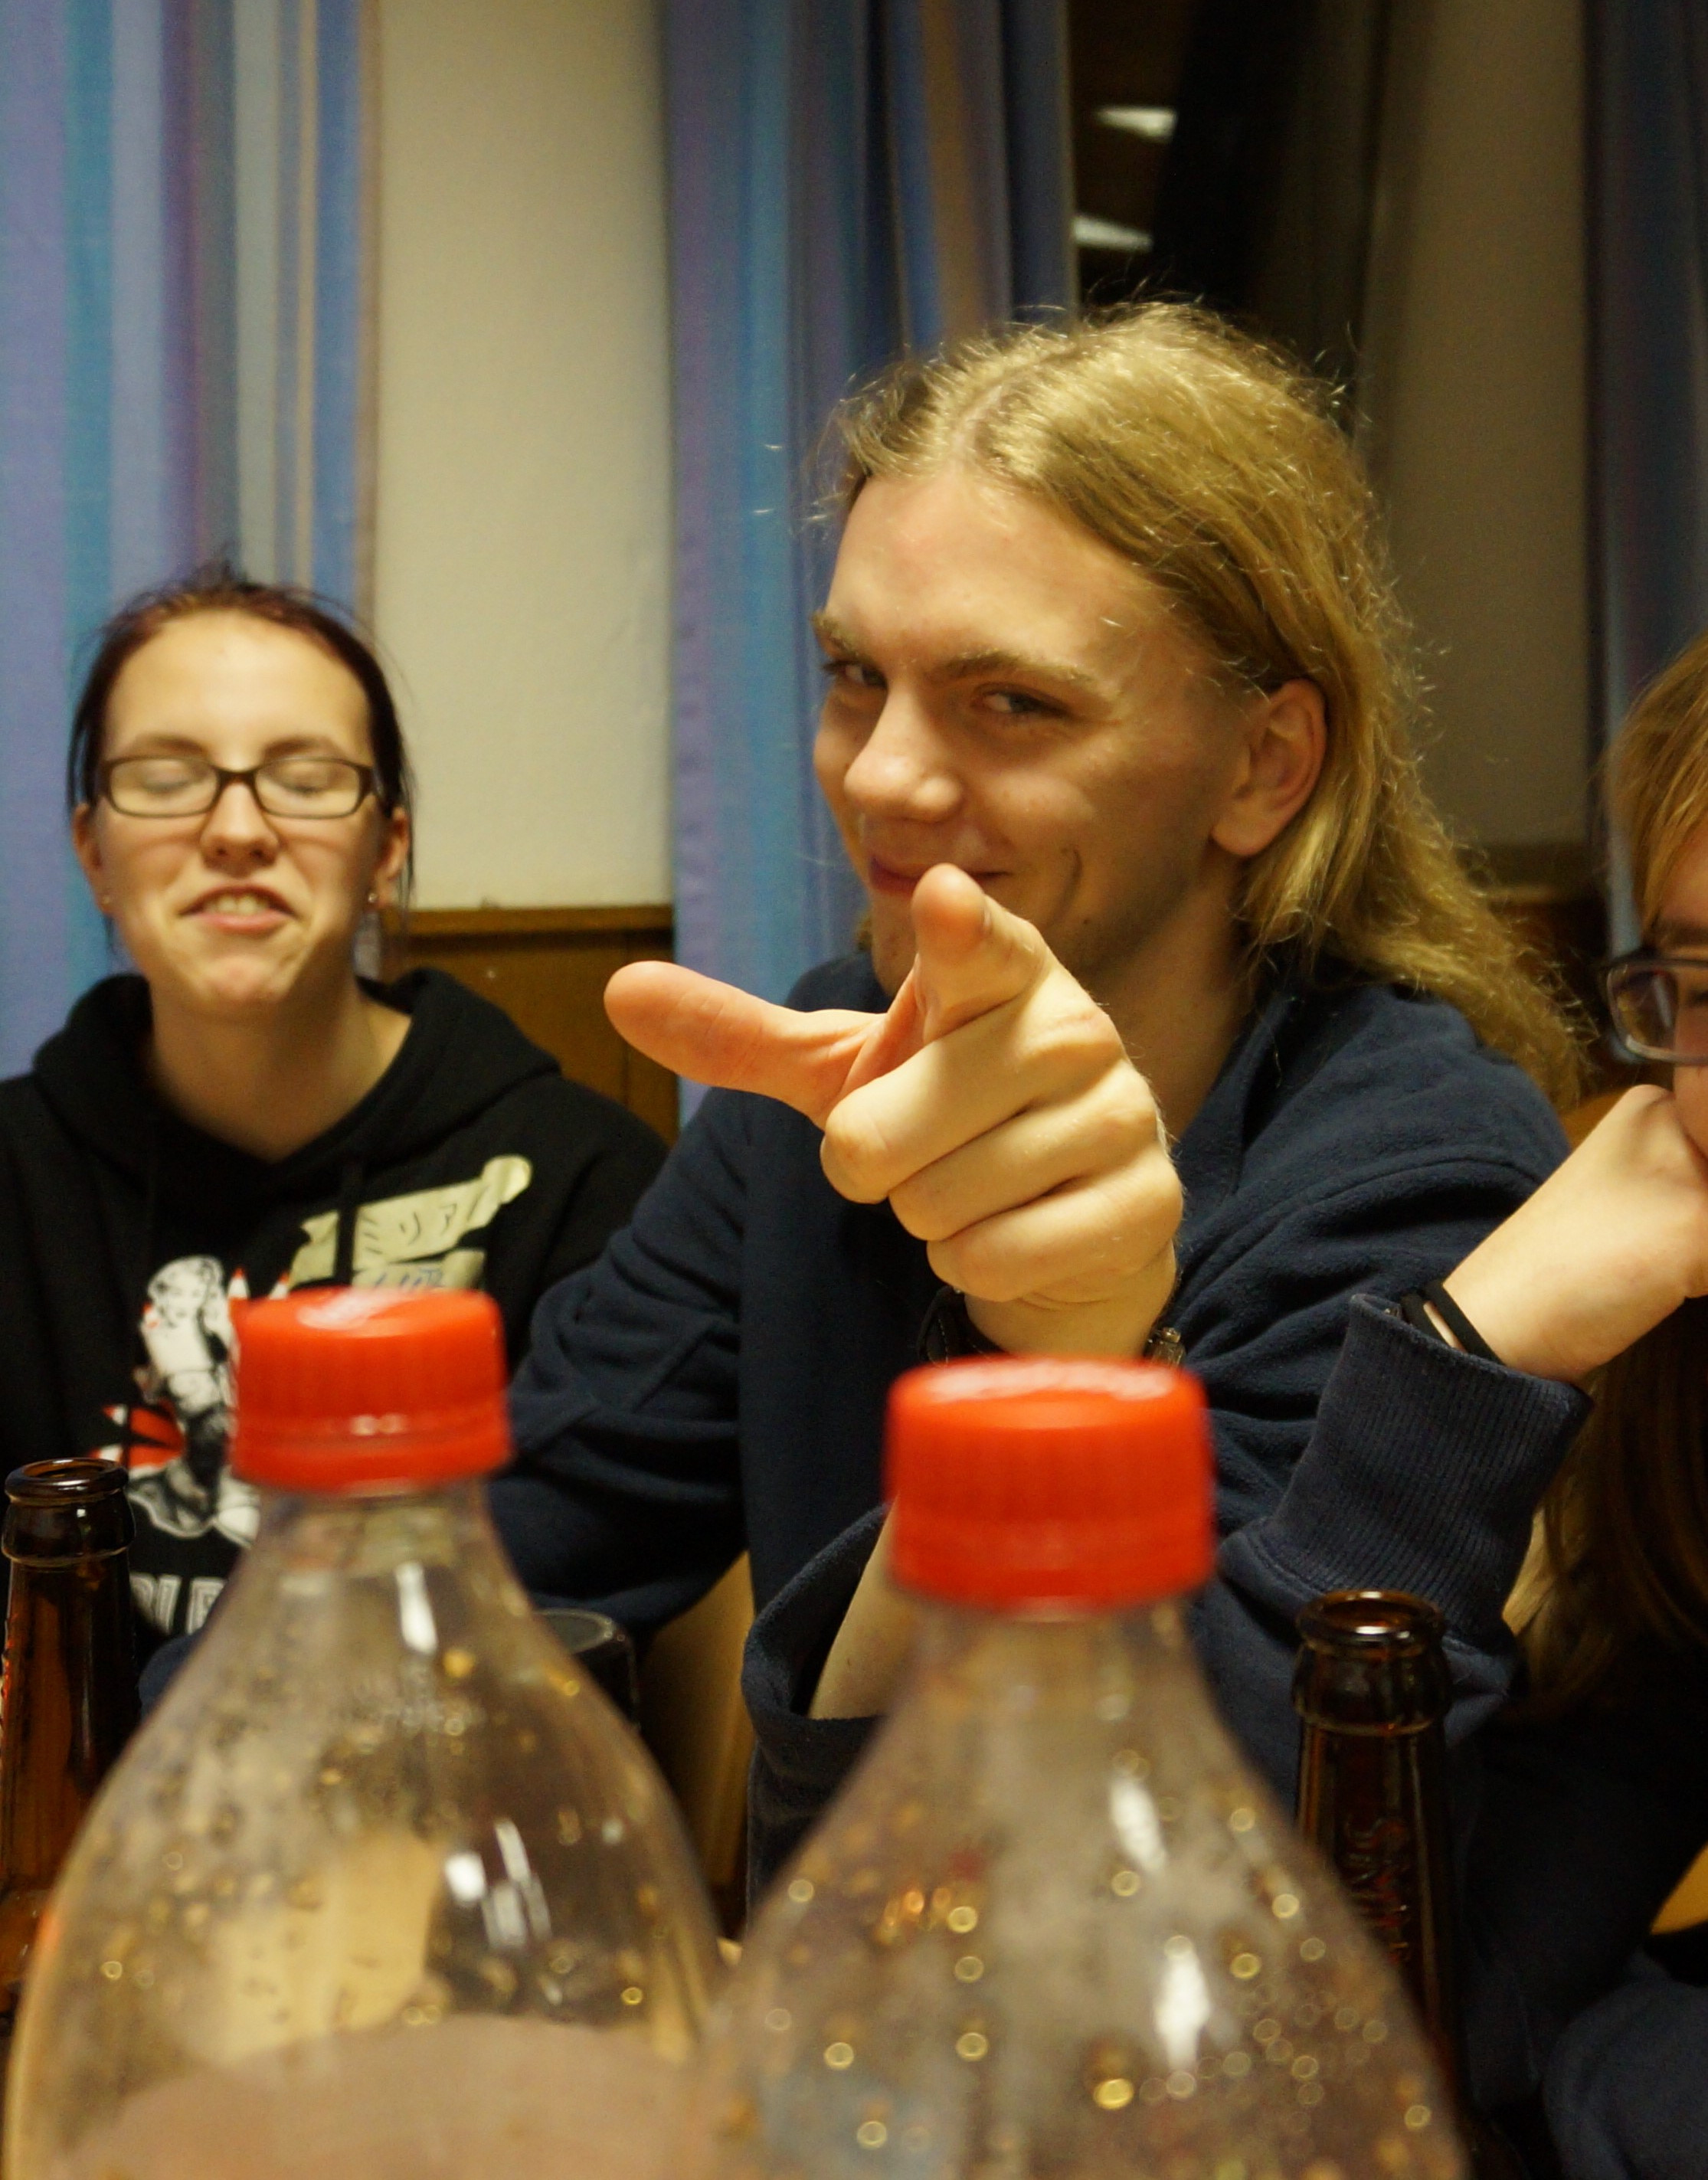
\includegraphics[width=\columnwidth]{res/erstiwe/valentin_finger_cropped.jpg}
\end{center}
\end{multicols*}
